\documentclass[onecolumn, 12pt, a4paper]{article}
\usepackage[a4paper,left = 2.5cm,right = 2.5cm, top = 2.5cm, bottom = 2.5cm]{geometry}
\usepackage{physics}
\usepackage{amsmath}
\usepackage{graphicx}
\usepackage{caption}
 
\author{
  George Herbert\\
  \texttt{cj19328@bristol.ac.uk}
}

\title{An Unknown Signal Report}
\begin{document}

\maketitle

\begin{abstract}
    This report demonstrates my understanding of the methods I have 
    used, the results results I have obtained and my understanding
    of issues such as overfitting for the `An Unknown Signal'
    coursework.
\end{abstract}

\section{Equations for linear regression}

For a set of points that lie along a line with Gaussian noise 
$\vb{y} = \vb{X}\vb{w} + \vb{\epsilon}$ where $\epsilon_{i} \sim \mathcal{N}(0, \sigma^{2})$,
the maximum likelihood esimation of $\vb{w}$ is equivalent to
the least square error estimation and is given by the equation:
\[
    \vb{\hat{w}} = (\vb{X}^{T}\vb{X})^{-1}\vb{X}^{T}\vb{y}.
\]
This equation is implemented in my code as the following
method:
\begin{verbatim}
def regressionNormalEquation(self, X, y):
    return np.linalg.inv(X.T @ X) @ X.T @ y
\end{verbatim}

$\vb{X}$ can take one of the following
three forms:
\[
\vb{X} =
\begin{bmatrix}
    x_{1} & 1 \\
    \vdots & \vdots \\
    x_{20} & 1 \\
\end{bmatrix}
\quad
\vb{X} =
\begin{bmatrix}
    x_{1}^{n} & x_{1}^{n-1} & \dots & 1 \\
    \vdots & \vdots & \ddots & \vdots \\
    x_{20}^{n} & x_{20}^{n-1} & \dots & 1 \\
\end{bmatrix}
\quad
\vb{X} =
\begin{bmatrix}
    f(x_{1}) & 1 \\
    \vdots & \vdots \\
    f(x_{20}) & 1 \\
\end{bmatrix}
\]
depending on whether the line is linear, polynomial of degree $n$,
or the unknown function $f$, respectively.

\section{Choice of polynomial degree}

\begin{table}[htbp]
    \begin{center}
        \caption{\label{tab:degree.py}Section of the output from `\texttt{degree.py}'}
    \begin{tabular}{l l l l} 
        \hline\hline
        Filename & Line segment & Polynomial degree & Cross-validation error \\ [0.5ex] 
        \hline
        basic\_3.csv & 0 & 2 & 7.3947610358752875 \\ 
        basic\_3.csv & 0 & 3 & 1.2989585613760917e-23 \\
        \vdots & \vdots & \vdots & \vdots \\
        adv\_3.csv & 5 & 9 & 318.8443359827487 \\
        adv\_3.csv & 5 & 10 & 279.2750683133305 \\
        \hline
    \end{tabular}
    \end{center}
\end{table}

Having created a program, `\texttt{display.py}', to visualise
the graphs, I drew up a list of line segments that appeared to
be nonlinear.
Then, I created a program, `\texttt{degree.py}', that calculated
the cross-validation error for each of these line segments
when trained using a model with a polynomial of degree 2,
to a polynomial of degree 10. A small section of the output
from this program is shown in Table \ref{tab:degree.py}.

Having analysed the output, it was clear that a large
proportion of the nonlinear signals had their lowest
cross-validation error when fitted with a polynomial of degree
3.
This indicated that the polynomial line segments in 
the unknown signal are cubic.

\begin{figure}[htbp]
\centering
\begin{minipage}[b]{.49\textwidth}
    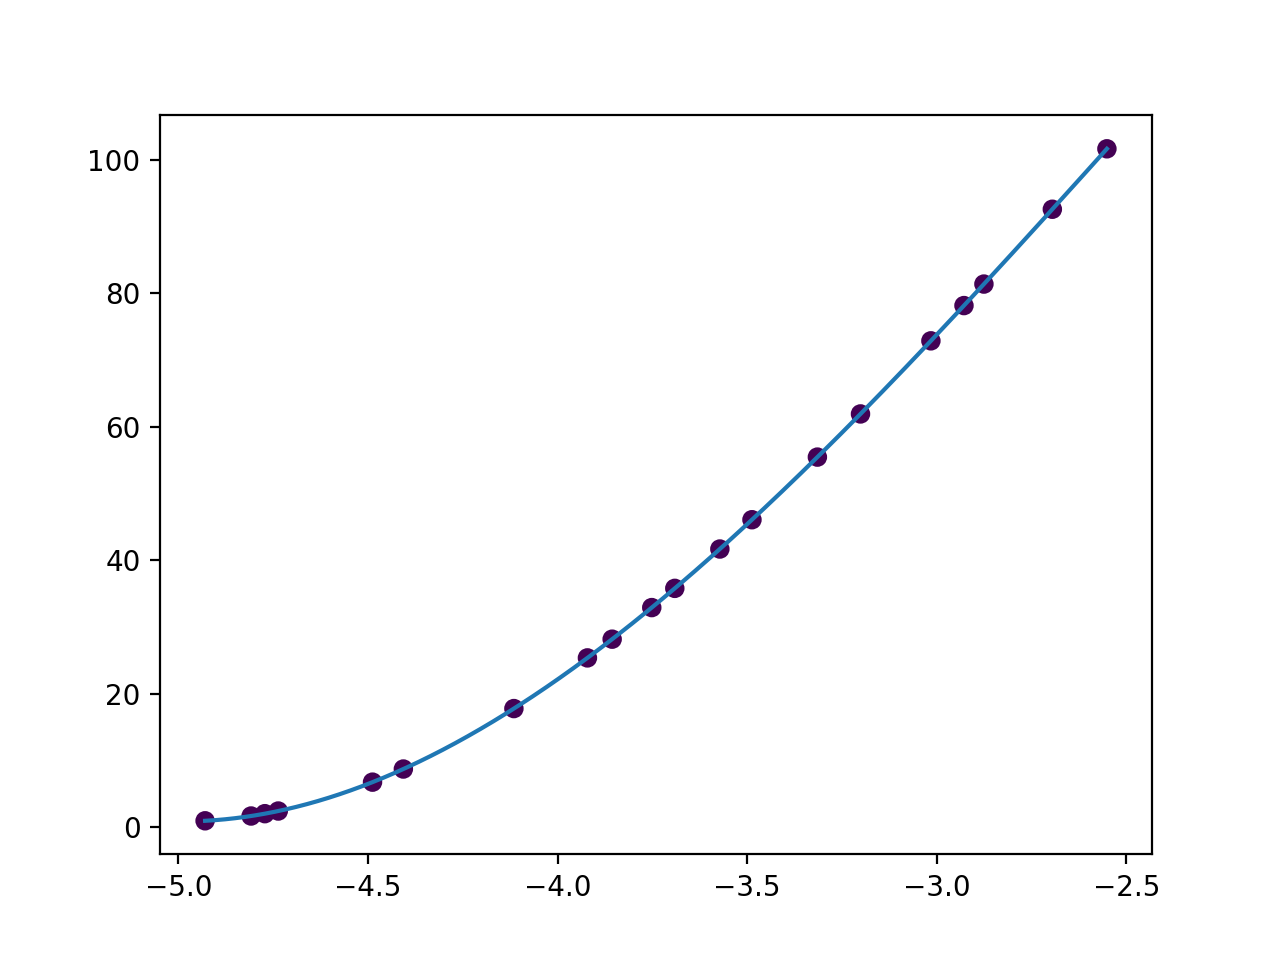
\includegraphics[width=\textwidth]{images/basic_3.png}
    \caption{Plot for `\texttt{basic\_3.csv}'}
    \label{fig:basic_3.csv}
\end{minipage}
\hfill
\begin{minipage}[b]{.49\textwidth}
    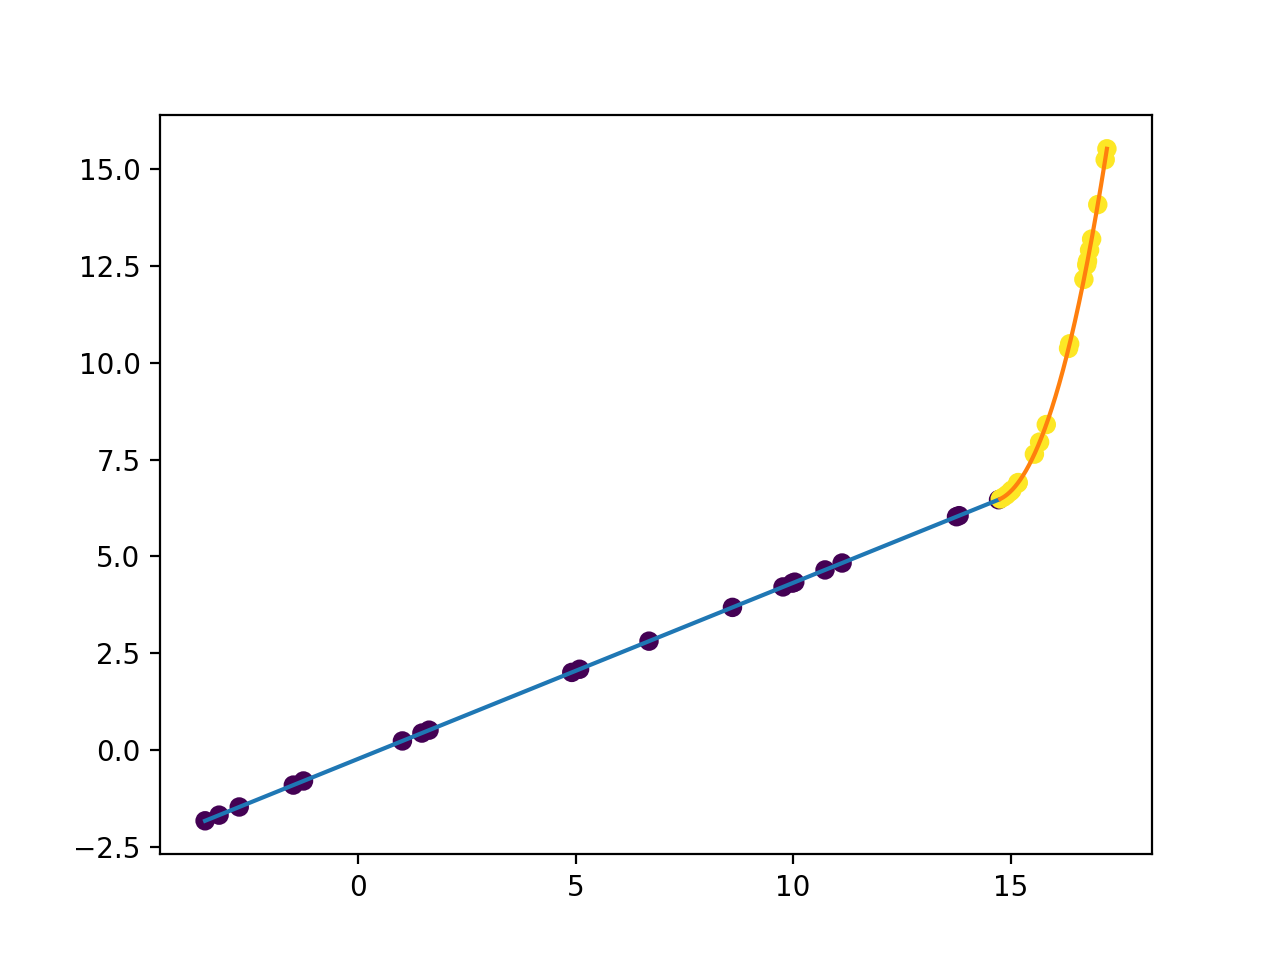
\includegraphics[width=\textwidth]{images/basic_4.png}
    \caption{Plot for `\texttt{basic\_4.csv}'}
    \label{fig:basic_4.csv}
\end{minipage}
\end{figure}

Having incorporated cubic regression into my `\texttt{lsr.py}'
least-squares regression program, I ran the program on
the `\texttt{basic\_3.csv}' and `\texttt{basic\_4.csv}'
unknown signals;
the outputs are shown in Figure \ref{fig:basic_3.csv}
and Figure \ref{fig:basic_4.csv} respectively.
The lines being a near-perfect fit allowed me to
visually validate that a cubic polynomial is reasonable.

\section{Choice of unknown function}

Using my `\texttt{display.py}' program to visualise the
signals, I produced a list of potential functions that could
be used to produce the line segments, based on their shapes:
$\vb{w}_{1}sin(x) + \vb{w}_{2}$,
$\vb{w}_{1}cos(x) + \vb{w}_{2}$,
$\vb{w}_{1}tan(x) + \vb{w}_{2}$ and
$\vb{w}_{1}e^{x} + \vb{w}_{2}$.

I then created a program `\texttt{unknown.py}' that
calculated the cross-validation error for each of the
nonlinear line segments previously identified, when
trained using each of the potential unknown functions.
The values of which were outputted in a table---similar 
to that used to determine the degree of the polynomial.

Having analysed the cross-validation errors, it was clear
that all nonlinear signals that were likely not
a cubic polynomial, had their minimum cross-validation
error when trained to fit the function
$\vb{w}_{1}sin(x) + \vb{w}_{2}$.

\begin{figure}[htbp]
\centering
\begin{minipage}[b]{.49\textwidth}
    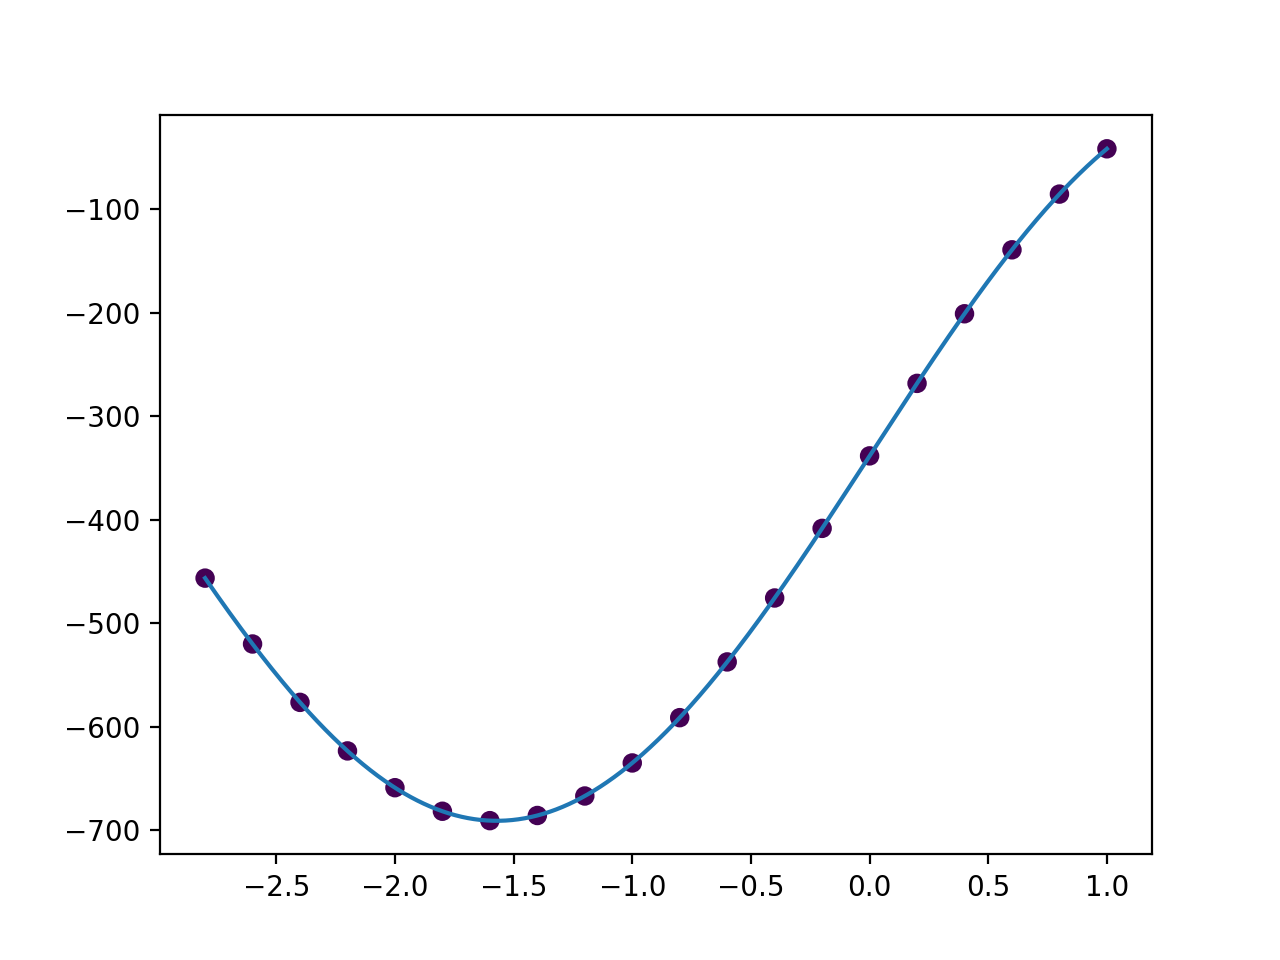
\includegraphics[width=\textwidth]{images/basic_5.png}
    \caption{Plot for `\texttt{basic\_5.csv}'}
    \label{fig:basic_5.csv}
\end{minipage}
\hfill
\begin{minipage}[b]{.49\textwidth}
    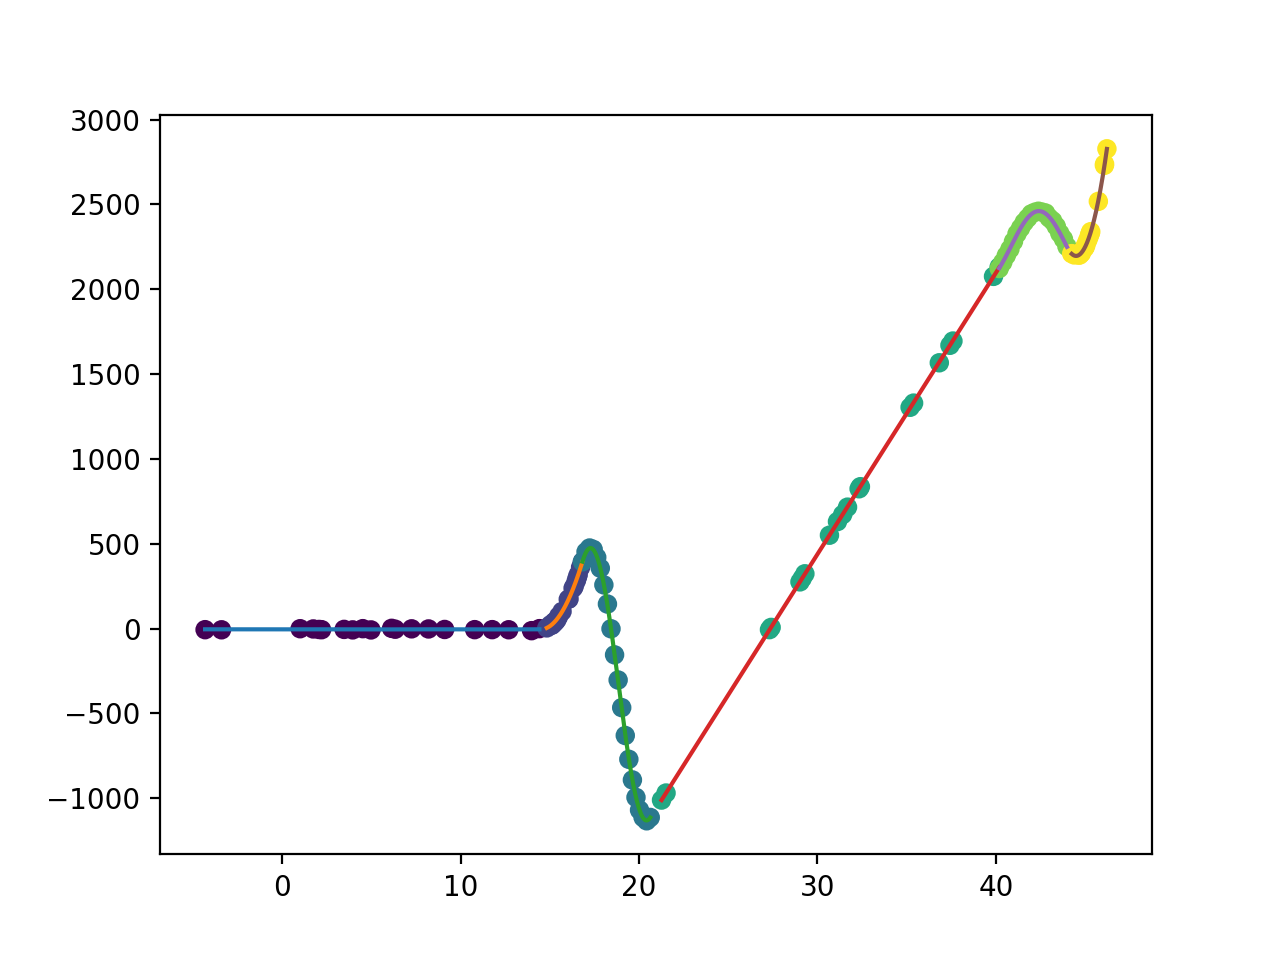
\includegraphics[width=\textwidth]{images/adv_3.png}
    \caption{Plot for `\texttt{adv\_3.csv}'}
    \label{fig:adv_3.csv}
\end{minipage}
\end{figure}

Having incorporated regression to fit a function of the
form $\vb{w}_{1}sin(x) + \vb{w}_{2}$ into my 
`\texttt{lsr.py}'
least-squares regression program, I ran the program on
the `\texttt{basic\_5.csv}' and `\texttt{adv\_3.csv}'
unknown signals;
the outputs are shown in Figure \ref{fig:basic_5.csv}
and Figure \ref{fig:adv_3.csv} respectively.
The lines being a near-perfect fit allowed me to
visually validate that the unknown function is of
the form $\vb{w}_{1}sin(x) + \vb{w}_{2}$.

\section{Model selection}

Overfitting occurs when a machine learning algorithm
produces a model that has learnt the noise in the data
as if it represents the structure of the underlying
model \cite{MSMI}.
In the case of linear regression, overfitting is most
likely to occur by producing a model with too complex a function
type, such that it would fail to predict future observations.

To prevent overfitting, I have used leave-one-out
cross-validation when producing a model for each 20-point
line segment. Leave-one-out cross-validation is 
an extreme case of $k$-fold cross validation
such that $k = n$, where
$n$ is the number of data-points (in this case 20).
Despite being computationally expensive, I believe that
leave-one-out cross-validation is an appropriate technique
to prevent overfitting in this case,
owing to the limited sample size of each line segment.

Leave-one-out cross-validation involves using each of
the 20 data-points exactly once as validation data for a model
trained using the other 19 data-points. 
The cross-validation error for each function type is calculated
as follows \cite{Stanford}:
\[
    CV_{(n)} = \frac{1}{n} \sum_{i = 1}^{n} (y_{i} - \hat{y}^{(-i)})^{2}
\]
where
$n$ is the number of datapoints in a line segment (i.e. 20);
$y_{i}$ is the actual $y$-value for the $i$-th datapoint;
and $\hat{y}^{(-i)}$ is the predicted $y$-value for the $i$-th
datapoint, when trained without using the $i$-th sample.

The function type with the lowest cross-validation error is then selected.

\section{Optimisations and improvements}

To begin with,
computing the matrix inverse using the \texttt{np.linalg.inv}
method is computationally expensive and unncessary.
Instead, given $\vb{X}$ and $\vb{y}$, the maximum likelihood
estimation could be computed directly as follows:
\texttt{np.linalg.solve(X.T @ X, @ X.T @ y)}.
This would be faster, as \texttt{np.linalg.inv}
computes the inverse of a matrix $\vb{A}$ by solving for $\vb{A}^{-1}$
in $\vb{AA^{-1} = I}$ \cite{StackOverflow}.
Thus, there would be a performance benefit by solving for
$\vb{\hat{w}}$ in
$\vb{X}^{T} \vb{X} \vb{\hat{w}} = \vb{X}^{T} \vb{y}$ directly.

Another computationally expensive operation in my
algorithm is that used to calculate the cross-validation error 
using leave-one-out cross-validation.
This is because it involves
fitting the model and calculating the sum squared error
$n$ times. 
Instead, there exists a faster method I could have
adopted that involves calculating the leverage.
Despite this, I opted not to include this method; 
owing to the fact that my program as it
currently stands can be easily adapted to use $k$-fold
cross-validation for any value of $k$ that is a factor of 20
by changing the constant `\texttt{K}' in the code.

\section{Testing}

I created a file `\texttt{test.py}' to test each of the
methods in my program using the
\texttt{unittest} unit testing framework.

\begin{thebibliography}{9}

    \bibitem{MSMI}
    Burnham, K. P. and Anderson, D. R. (2002)
    \textit{Model Selection and Multimodel Inference}.
    2nd ed. Springer-Verlag.

    \bibitem{Stanford}
    Taylor, J. (2020)
    \textit{Leave one out cross-validation (LOOCV) --- STATS 202}
    https://web.stanford.edu/class/stats202/notes/Resampling/LOOCV.html

    \bibitem{StackOverflow}
    Muldal, A. (2017)
    \textit{Why does numpy.linalg.solve() offer more precise matrix inversions than numpy.linalg.inv()?}
    https://stackoverflow.com/a/31257909/8540479



\end{thebibliography}
    

\end{document}
